\documentclass[crop,tikz]{standalone}
\usepackage{amsfonts}
\usetikzlibrary{shapes}
\usetikzlibrary{arrows}
\usetikzlibrary{positioning}
\begin{document}
 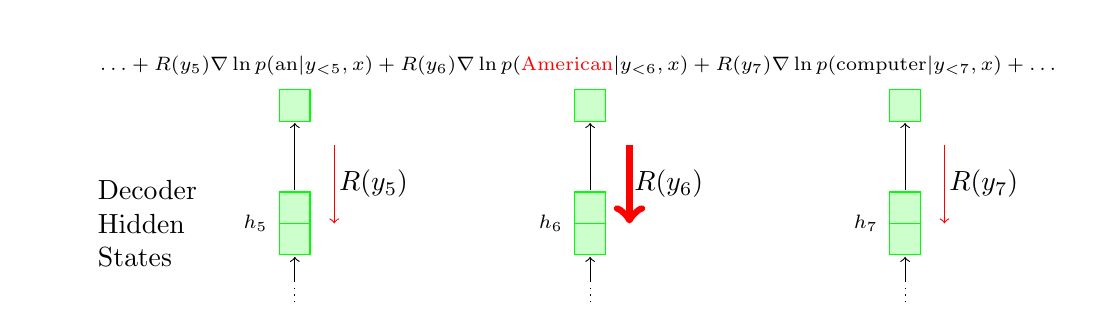
\begin{tikzpicture}[
    record/.style={rectangle,draw=black,anchor=north west,text width=42mm,
                   font=\scriptsize},
    beam/.style={rectangle,draw=black,anchor=north west,text width=36mm,
                 font=\scriptsize},
    table/.style={anchor=north west,rotate=90,font=\tiny},
    dot/.style={circle,draw=black,fill=white,inner sep=.75pt},
  hid/.style 2 args={
    rectangle split,
    draw=#2,
    rectangle split parts=#1,
    fill=#2!20,
    outer sep=.25mm},
  mlp/.style 2 args={
    rectangle split,
    rectangle split horizontal,
    draw=#2,
    rectangle split parts=#1,
    fill=#2!20,
b
    outer sep=.25mm}
 ]

%\node[anchor=west] at (2,5) {Speaker: $y \sim p(\cdot|x)\quad\quad\quad\quad$ Listener: $ \hat{x} \sim q(\cdot|y)$};
%\node[anchor=west] at (2,4.5) {Reward: $R(y) = q(x|y)\quad\quad$~ Objective: $  \mathcal{L} = \mathbb{E}_{y\sim p(\cdot|x) }\left[ R(y) \right]  $};

\node[text width=2cm] at (1.75, 1) {Decoder Hidden States};

%\draw[black] (0,0) rectangle (11,6);
\node[anchor=west] at (-0.15,3) {\scriptsize ${\color{white}R(y) \Big[} \ldots 
+  R(y_5) \nabla\ln p(\textrm{an}|y_{<5},x)
+  R(y_6) \nabla\ln p(\textrm{\color{red}American}|y_{<6},x)
+  R(y_7) \nabla\ln p(\textrm{computer}|y_{<7},x) + \ldots \color{white}{\Big]}$};


 \node[hid={2}{green}] (h1) at (3.25, 1) {};
 \node (s) at (2.75, 1) {\scriptsize $h_5$};
  \draw[->,red] (3.75, 2) to (3.75, 1);
\node at (4.25, 1.5) {$R(y_5)$};
  \draw[-,black,dotted] (3.25, 0) to (3.25, .25);
  \draw[->,black] (3.25, .25) to (h1.south);
 \node[hid={1}{green}] (p1) at (3.25, 2.5) {};
\draw[->,black] (h1.north) to (p1.south);



 \node[hid={2}{green}] (h2) at (7, 1) {};
 \node (s) at (6.5, 1) {\scriptsize $h_6$};
  \draw[->,red,line width=1mm] (7.5, 2) to (7.5, 1);
\node at (8, 1.5) {$R(y_6)$};
  \draw[-,black,dotted] (7, 0) to (7, .25);
  \draw[->,black] (7, .25) to (h2.south);
 \node[hid={1}{green}] (p2) at (7, 2.5) {};
\draw[->,black] (h2.north) to (p2.south);

 \node[hid={2}{green}] (h3) at (11, 1) {};
 \node (lbl3) at (10.5, 1) {\scriptsize $h_7$};
  \draw[->,red] (11.5, 2) to (11.5, 1);
\node at (12, 1.5) {$R(y_7)$};
  \draw[-,black,dotted] (11, 0) to (11, .25);
  \draw[->,black] (11, .25) to (h3.south);
 \node[hid={1}{green}] (p3) at (11, 2.5) {};
\draw[->,black] (h3.north) to (p3.south);

 \end{tikzpicture}
\end{document}
